
\documentclass[a4paper,11pt]{article}
\usepackage[a4paper, margin=8em]{geometry}

% usa i pacchetti per la scrittura in italiano
\usepackage[french,italian]{babel}
\usepackage[T1]{fontenc}
\usepackage[utf8]{inputenc}
\frenchspacing 

% usa i pacchetti per la formattazione matematica
\usepackage{amsmath, amssymb, amsthm, amsfonts}

% usa altri pacchetti
\usepackage{gensymb}
\usepackage{hyperref}
\usepackage{standalone}

\usepackage{colortbl}

\usepackage{xstring}
\usepackage{karnaugh-map}

% imposta il titolo
\title{Specification and Simulation of Digital Systems notes}
\author{Luca Seggiani}
\date{2026}

% imposta lo stile
% usa helvetica
\usepackage[scaled]{helvet}
% usa palatino
\usepackage{palatino}
% usa un font monospazio guardabile
\usepackage{lmodern}

\renewcommand{\rmdefault}{ppl}
\renewcommand{\sfdefault}{phv}
\renewcommand{\ttdefault}{lmtt}

% circuiti
\usepackage{circuitikz}
\usetikzlibrary{babel}

% testo cerchiato
\newcommand*\circled[1]{\tikz[baseline=(char.base)]{
            \node[shape=circle,draw,inner sep=2pt] (char) {#1};}}

% disponi il titolo
\makeatletter
\renewcommand{\maketitle} {
	\begin{center} 
		\begin{minipage}[t]{.8\textwidth}
			\textsf{\huge\bfseries \@title} 
		\end{minipage}%
		\begin{minipage}[t]{.2\textwidth}
			\raggedleft \vspace{-1.65em}
			\textsf{\small \@author} \vfill
			\textsf{\small \@date}
		\end{minipage}
		\par
	\end{center}

	\thispagestyle{empty}
	\pagestyle{fancy}
}
\makeatother

% disponi teoremi
\usepackage{tcolorbox}
\newtcolorbox[auto counter, number within=section]{theorem}[2][]{%
	colback=blue!10, 
	colframe=blue!40!black, 
	sharp corners=northwest,
	fonttitle=\sffamily\bfseries, 
	title=Theorem~\thetcbcounter: #2, 
	#1
}

% disponi definizioni
\newtcolorbox[auto counter, number within=section]{definition}[2][]{%
	colback=red!10,
	colframe=red!40!black,
	sharp corners=northwest,
	fonttitle=\sffamily\bfseries,
	title=Definition~\thetcbcounter: #2,
	#1
}

% disponi codice
\usepackage{listings}
\usepackage[table]{xcolor}

\definecolor{codegreen}{rgb}{0,0.6,0}
\definecolor{codegray}{rgb}{0.5,0.5,0.5}
\definecolor{codepurple}{rgb}{0.58,0,0.82}
\definecolor{backcolour}{rgb}{0.95,0.95,0.92}

\lstdefinestyle{codestyle}{
		backgroundcolor=\color{black!5}, 
		commentstyle=\color{codegreen},
		keywordstyle=\bfseries\color{magenta},
		numberstyle=\sffamily\tiny\color{black!60},
		stringstyle=\color{green!50!black},
		basicstyle=\ttfamily\footnotesize,
		breakatwhitespace=false,         
		breaklines=true,                 
		captionpos=b,                    
		keepspaces=true,                 
		numbers=left,                    
		numbersep=5pt,                  
		showspaces=false,                
		showstringspaces=false,
		showtabs=false,                  
		tabsize=2
}

\lstdefinestyle{shellstyle}{
		backgroundcolor=\color{black!5}, 
		basicstyle=\ttfamily\footnotesize\color{black}, 
		commentstyle=\color{black}, 
		keywordstyle=\color{black},
		numberstyle=\color{black!5},
		stringstyle=\color{black}, 
		showspaces=false,
		showstringspaces=false, 
		showtabs=false, 
		tabsize=2, 
		numbers=none, 
		breaklines=true
}

\lstdefinelanguage{x86}{ 
  keywords={AAA, AAD, AAM, AAS, ADC, ADCB, ADCW, ADCL, ADD, ADDB, ADDW, ADDL, AND, ANDB, ANDW, ANDL,
        ARPL, BOUND, BSF, BSFL, BSFW, BSR, BSRL, BSRW, BSWAP, BT, BTC, BTCB, BTCW, BTCL, BTR, 
        BTRB, BTRW, BTRL, BTS, BTSB, BTSW, BTSL, CALL, CBW, CDQ, CLC, CLD, CLI, CLTS, CMC, CMP,
        CMPB, CMPW, CMPL, CMPS, CMPSB, CMPSD, CMPSW, CMPXCHG, CMPXCHGB, CMPXCHGW, CMPXCHGL,
        CMPXCHG8B, CPUID, CWDE, DAA, DAS, DEC, DECB, DECW, DECL, DIV, DIVB, DIVW, DIVL, ENTER,
        HLT, IDIV, IDIVB, IDIVW, IDIVL, IMUL, IMULB, IMULW, IMULL, IN, INB, INW, INL, INC, INCB,
        INCW, INCL, INS, INSB, INSD, INSW, INT, INT3, INTO, INVD, INVLPG, IRET, IRETD, JA, JAE,
        JB, JBE, JC, JCXZ, JE, JECXZ, JG, JGE, JL, JLE, JMP, JNA, JNAE, JNB, JNBE, JNC, JNE, JNG,
        JNGE, JNL, JNLE, JNO, JNP, JNS, JNZ, JO, JP, JPE, JPO, JS, JZ, LAHF, LAR, LCALL, LDS,
        LEA, LEAVE, LES, LFS, LGDT, LGS, LIDT, LMSW, LOCK, LODSB, LODSD, LODSW, LOOP, LOOPE,
        LOOPNE, LSL, LSS, LTR, MOV, MOVB, MOVW, MOVL, MOVSB, MOVSD, MOVSW, MOVSX, MOVSXB,
        MOVSXW, MOVSXL, MOVZX, MOVZXB, MOVZXW, MOVZXL, MUL, MULB, MULW, MULL, NEG, NEGB, NEGW,
        NEGL, NOP, NOT, NOTB, NOTW, NOTL, OR, ORB, ORW, ORL, OUT, OUTB, OUTW, OUTL, OUTSB, OUTSD,
        OUTSW, POP, POPL, POPW, POPB, POPA, POPAD, POPF, POPFD, PUSH, PUSHL, PUSHW, PUSHB, PUSHA, 
        RCLL, RCR, RCRB, RCRW, RCRL, RDMSR, RDPMC, RDTSC, REP, REPE, REPNE, RET, ROL, ROLB, ROLW,
        ROLL, ROR, RORB, RORW, RORL, SAHF, SAL, SALB, SALW, SALL, SAR, SARB, SARW, SARL, SBB,
        SBBB, SBBW, SBBL, SCASB, SCASD, SCASW, SETA, SETAE, SETB, SETBE, SETC, SETE, SETG, SETGE,
        SETL, SETLE, SETNA, SETNAE, SETNB, SETNBE, SETNC, SETNE, SETNG, SETNGE, SETNL, SETNLE,
        SETNO, SETNP, SETNS, SETNZ, SETO, SETP, SETPE, SETPO, SETS, SETZ, SGDT, SHL, SHLB, SHLW,
        SHLL, SHLD, SHR, SHRB, SHRW, SHRL, SHRD, SIDT, SLDT, SMSW, STC, STD, STI, STOSB, STOSD,
        STOSW, STR, SUB, SUBB, SUBW, SUBL, TEST, TESTB, TESTW, TESTL, VERR, VERW, WAIT, WBINVD,
        XADD, XADDB, XADDW, XADDL, XCHG, XCHGB, XCHGW, XCHGL, XLAT, XLATB, XOR, XORB, XORW, XORL},
  keywordstyle=\color{blue}\bfseries,
  ndkeywordstyle=\color{darkgray}\bfseries,
  identifierstyle=\color{black},
  sensitive=false,
  comment=[l]{\#},
  morecomment=[s]{/*}{*/},
  commentstyle=\color{purple}\ttfamily,
  stringstyle=\color{red}\ttfamily,
  morestring=[b]',
  morestring=[b]"
}

\lstdefinelanguage{riscv}{
  keywords={
    LUI, AUIPC,
    JAL, JALR,
    BEQ, BNE, BLT, BGE, BLTU, BGEU,
    LB, LH, LW, LBU, LHU, LD,
    SB, SH, SW, SD,
    ADDI, SLTI, SLTIU, XORI, ORI, ANDI,
    SLLI, SRLI, SRAI,
    ADD, SUB, SLL, SLT, SLTU, XOR, SRL, SRA, OR, AND,
    ADDIW, SLLIW, SRLIW, SRAIW,
    ADDW, SUBW, SLLW, SRLW, SRAW,
    MUL, MULH, MULHSU, MULHU, DIV, DIVU, REM, REMU,
    MULW, DIVW, DIVUW, REMW, REMUW,
    LR.W, SC.W, AMOSWAP.W, AMOADD.W, AMOXOR.W,
    AMOAND.W, AMOOR.W, AMOMIN.W, AMOMAX.W,
    AMOMINU.W, AMOMAXU.W,
    LR.D, SC.D, AMOSWAP.D, AMOADD.D, AMOXOR.D,
    AMOAND.D, AMOOR.D, AMOMIN.D, AMOMAX.D,
    AMOMINU.D, AMOMAXU.D,
    FLW, FSW,
    FMADD.S, FMSUB.S, FNMSUB.S, FNMADD.S,
    FADD.S, FSUB.S, FMUL.S, FDIV.S, FSQRT.S,
    FSGNJ.S, FSGNJN.S, FSGNJX.S,
    FMIN.S, FMAX.S,
    FCVT.W.S, FCVT.WU.S, FCVT.S.W, FCVT.S.WU,
    FMV.X.W, FMV.W.X,
    FEQ.S, FLT.S, FLE.S,
    FLD, FSD,
    FMADD.D, FMSUB.D, FNMSUB.D, FNMADD.D,
    FADD.D, FSUB.D, FMUL.D, FDIV.D, FSQRT.D,
    FSGNJ.D, FSGNJN.D, FSGNJX.D,
    FMIN.D, FMAX.D,
    FCVT.W.D, FCVT.WU.D, FCVT.D.W, FCVT.D.WU,
    FCVT.S.D, FCVT.D.S,
    FMV.X.D, FMV.D.X,
    FEQ.D, FLT.D, FLE.D,
    CSRRW, CSRRS, CSRRC,
    CSRRWI, CSRRSI, CSRRCI,
    FENCE.I,
    FENCE,
    ECALL, EBREAK,
    MRET, SRET, URET,
    WFI,
    SFENCE.VMA,
    NOP, LI, LA, MV,
    NOT, NEG, NEGW,
    SEQZ, SNEZ, SLTZ, SGTZ,
    BEQZ, BNEZ, BLEZ, BGEZ, BLTZ, BGTZ,
    BGT, BLE, BGTU, BLEU,
    J, JR, RET,
    CALL, TAIL,
    RDINSTRET, RDCYCLE, RDTIME,
    CSRR, CSRW, CSRS, CSRC,
    CSRWI, CSRSI, CSRCI
  },
  keywordstyle=\color{blue}\bfseries,
  ndkeywordstyle=\color{darkgray}\bfseries,
  identifierstyle=\color{black},
  sensitive=false,
  comment=[l]{\#},
  morecomment=[s]{/*}{*/},
  commentstyle=\color{purple}\ttfamily,
  stringstyle=\color{red}\ttfamily,
  morestring=[b]',
  morestring=[b]"
}

\lstdefinelanguage{arm}{
  keywords={
    ADC, ADD, AND, BIC, CMN, CMP, EOR, MOV, MVN,
    RSB, RSC, SBC, SUB, TST, TEQ,
    MLA, MLS, MUL, SMLAL, SMULL, UMLAL, UMULL,
    QADD, QSUB, QDADD, QDSUB,
    QADD16, QADD8, QASX, QSAX,
    QSUB16, QSUB8, QSAX, QSUBADDX,
    ASR, LSL, LSR, ROR, RRX,
    B, BL, BX, BLX,
    BXJ,
    BEQ, BNE, BCS, BHS, BCC, BLO,
    BMI, BPL, BVS, BVC,
    BHI, BLS, BGE, BLT, BGT, BLE,
    BAL,
    LDR, LDRB, LDRH, LDRSB, LDRSH,
    LDRD, LDM, LDMIA, LDMIB, LDMDA, LDMDB,
    LDRT, LDRBT, LDRHT, LDRSBT, LDRSHT,
    STR, STRB, STRH, STRD,
    STM, STMIA, STMIB, STMDA, STMDB,
    STRT, STRBT, STRHT,
    PUSH, POP,
    SWP, SWPB,
    REV, REV16, REVSH,
    BFC, BFI, BFXIL, SBFX, UBFX,
    CLZ,
    LDREX, LDREXB, LDREXH, LDREXD,
    STREX, STREXB, STREXH, STREXD,
    DMB, DSB, ISB,
    MCR, MCRR, MRC, MRRC,
    MRS, MSR,
    CPS, SETEND, SVC, BKPT,
    CLREX, WFE, WFI, SEV,
    YIELD, NOP,
    VLDR, VSTR,
    VMOV, VABS, VNEG,
    VADD, VSUB, VMUL, VDIV,
    VMLA, VMLS, VNMLA, VNMLS, VNMUL,
    VMAX, VMIN,
    VSQRT,
    VCMP, VCMPE,
    VCVT,
    VCLZ, VCLS,
    VAND, VORR, VEOR, VBIC, VMVN,
    VLD1, VLD2, VLD3, VLD4,
    VST1, VST2, VST3, VST4,
    ADR, ADCS, ADDS, SUBS, MOVS, ANDS, ORRS, EORS
  },
  keywordstyle=\color{blue}\bfseries,
  ndkeywordstyle=\color{darkgray}\bfseries,
  identifierstyle=\color{black},
  sensitive=false,
  comment=[l]{@},
  morecomment=[l]{;},
  morecomment=[s]{/*}{*/},
  commentstyle=\color{purple}\ttfamily,
  stringstyle=\color{red}\ttfamily,
  morestring=[b]',
  morestring=[b]"
}

\lstset{style=codestyle, language=C}

% disponi sezioni
\usepackage{titlesec}

\titleformat{\section}
	{\sffamily\Large\bfseries} 
	{\thesection}{1em}{} 
\titleformat{\subsection}
	{\sffamily\large\bfseries}   
	{\thesubsection}{1em}{} 
\titleformat{\subsubsection}
	{\sffamily\normalsize\bfseries} 
	{\thesubsubsection}{1em}{}

% tikz
\usepackage{tikz}

% float
\usepackage{float}

% grafici
\usepackage{pgfplots}
\pgfplotsset{width=10cm,compat=1.9}

% disponi alberi
\usepackage{forest}

\forestset{
	rectstyle/.style={
		for tree={rectangle,draw,font=\large\sffamily}
	},
	roundstyle/.style={
		for tree={circle,draw,font=\large}
	}
}

% disponi algoritmi
\usepackage{algorithm}
\usepackage{algorithmic}
\makeatletter
\renewcommand{\ALG@name}{Algorithm}
\makeatother

% disponi numeri di pagina
\usepackage{fancyhdr}
\fancyhf{} 
\fancyfoot[L]{\sffamily{\thepage}}

\makeatletter
\fancyhead[L]{\raisebox{1ex}[0pt][0pt]{\sffamily{\@title \ \@date}}} 
\fancyhead[R]{\raisebox{1ex}[0pt][0pt]{\sffamily{\@author}}}
\makeatother

\begin{document}
% sezione (data)
\section{Lesson 25-09-26}

% stili pagina
\thispagestyle{empty}
\pagestyle{fancy}

% testo
\subsection{Introduction to VHDL}

Let's start delving into the \textbf{VHDL} (\textit{VHSIC Hardware Description Language}) language.
There are 3 description styles in VHDL:
\begin{itemize}
	\item
	      Behavioral:
	      \begin{itemize}
		      \item Specifies only the behavior at a higher level of abstraction.
		      \item Does not imply any particular structure or technology.
	      \end{itemize}
	\item
	      Structural:
	      \begin{itemize}
		      \item Specifies more details.
		      \item Components used and the structure of the interconnection between the components are clearly specified.
		      \item At a low level of abstraction
	      \end{itemize}
	\item
	      Dataflow (\textit{Register Transfer Language} (\textbf{RTL})):
	      \begin{itemize}
		      \item Data path and control signals are specified.
		      \item System is described in terms of the data transfer between registers.
		      \item At an intermediate level of abstraction
	      \end{itemize}
\end{itemize}

We also note that VHDL's syntax is Ada-based, case insensitive.

\subsubsection{VHDL entities}

A simple VHDL file contains a \textbf{design entity}, comprised of:
\begin{itemize}
	\item An \textit{entity declaration};
	\item An \textit{architecture body}.
\end{itemize}

Let's look at a very simple entity declaration:

\begin{center}
	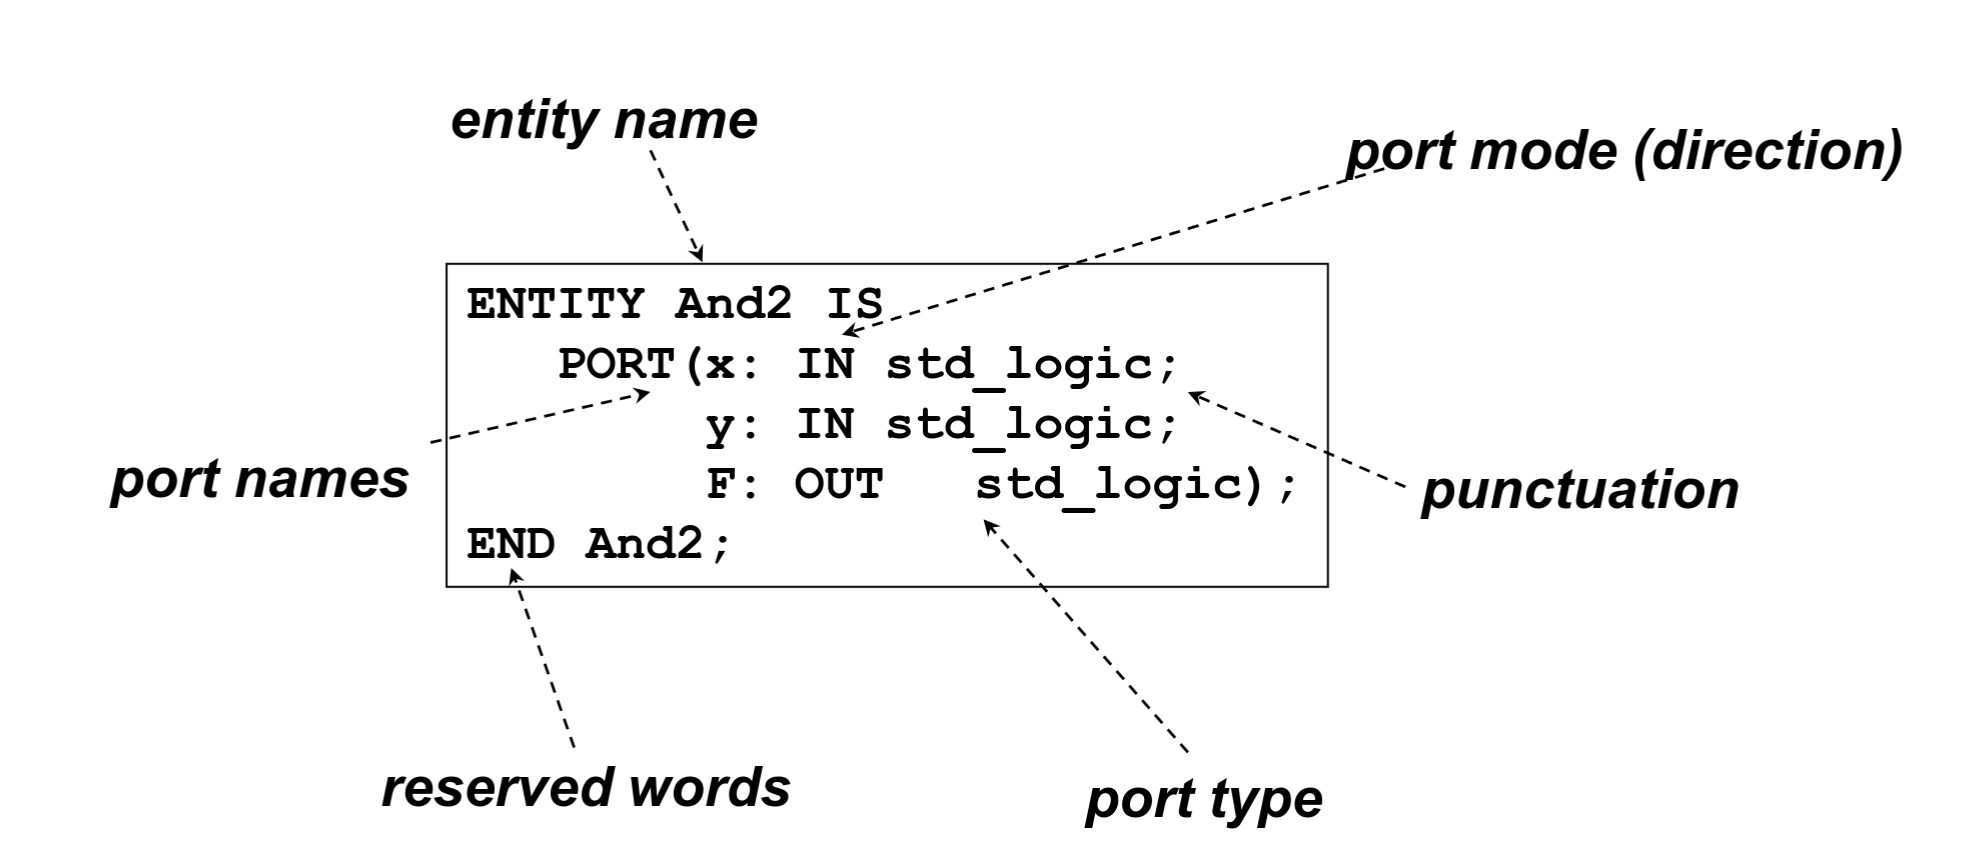
\includegraphics[scale=0.25]{../figures/entity_decl.png}
\end{center}

As we know the declaration gives a \textit{black box} view of the component, without its internal architecture.

\texttt{PORT} specifies a list of inputs and outputs of entity.
\begin{itemize}
	\item  \lstinline|x: IN std_logic|: port \texttt{x} is an input port of type \texttt{std\_logic};
	\item  \texttt{std\_logic}: short for "standard logic", a logical bit type (versus say an integer type), which can be '0' or '1' (more later);
	\item  Ports in list separated by semicolons.
\end{itemize}

A number of port modes are available:
\begin{itemize}
	\item IN: Used for a signal that is an input to an entity.
	\item OUT: Used for a signal that is an output from an entity. The value of the signal can not be used inside the entity. This means that in an assignment statement, the signal can appear only to the left of the <= operator.
	\item INOUT: Used for a signal that is both an input to an entity and an output from the entity.
	\item BUFFER: Used for a signal that is an output from an entity. The value of the signal can be used inside the entity, which means that in an assignment statement, the signal can appear both on the left and right sides of the <= operator.
\end{itemize}

BUFFER differs from INOUT because of the following:
\begin{itemize}
	\item It can’t have more than 1 source;
	\item The only signal connected to it is another BUFFER port or signal with at most 1 source.
\end{itemize}

\par\smallskip

\textbf{\textsf{Logic types}}: VHDL supports different data types for logic.
We'll mainly use \textbf{standard logic} as defined by IEEE 1164 standard (end of the 1980s).
\begin{itemize}
	\item Values for simulation: 'U' (unaffected), 'X' (unknown), 'Z' (high impedance), 'W' (weak unknown), 'L' (weak 0), 'H' (weak 1), '-' (don't care), 0, 1
	\item package \texttt{std\_logic\_1164}: it contains the enumerated types \texttt{std\_logic} and \texttt{std\_ulogic}. The main difference between \texttt{std\_logic} (standard logic) and  \texttt{std\_ulogic} (standard unresolved logic) is:
	      \begin{itemize}
		      \item \texttt{u} stands for \textit{unresolved} signal: it is illegal to force two values at the same time on a signal of type \texttt{std\_ulogic};
		      \item \texttt{std\_logic}: there exist resolution functions that define what happens when two values are forced at the same time on a signal.
	      \end{itemize}
\end{itemize}

\subsubsection{VHDL architectures}

An \textbf{architecture} defines an entity's inside --- an entity's functionality.
\begin{itemize}
	\item It describes the behavior or the inner implementation of an entity;
	\item There may be several architectures for the same entity (for simulation, but not for synthesis);
	\item Each architecture must be bound to an entity.
\end{itemize}

One way to describe architecture is thorugh \texttt{PROCESS}: a \texttt{PROCESS} takes in arguments, and reacts to changes of those arguments by producing an output value.
By \textit{reactive}, we mean that the process is idle until something happens to the arguments, at which points it \textit{reacts} by \textit{doing something}.
Because of this, the argument list is usually called the \textit{sensitivity list}.

Let's take, for instance:

\begin{tikzpicture}
	\node (code) {
		\begin{minipage}{\textwidth}
			\begin{lstlisting}[language=VHDL, style=codestyle]
ENTITY And2 IS
    PORT (x: IN std_logic;
    y: IN std_logic;
    F: OUT std_logic);
END And2;

ARCHITECTURE And2_beh OF And2 IS
BEGIN

    PROCESS(x, y) -- this is the process
    BEGIN
        F <= x AND y;
    END PROCESS;

END And2_beh;
\end{lstlisting}
		\end{minipage}
	};

	\node[anchor=center] at ([xshift=4.5cm,yshift=0cm]code.center) {
		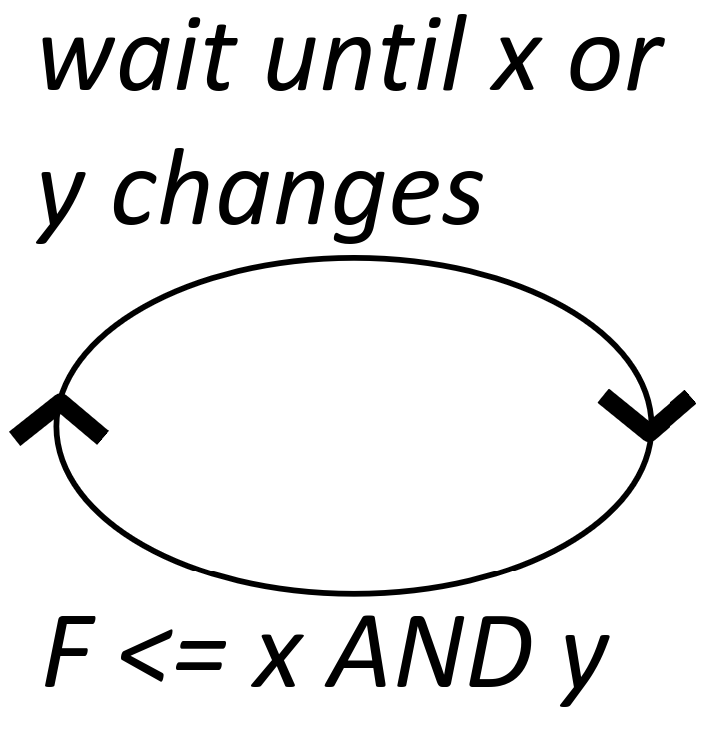
\includegraphics[scale=0.23]{../figures/proc_cycle.png}
	};
\end{tikzpicture}

If \texttt{x} and \texttt{y} change in the above example, the process sets the output $F$ to the logical AND of \texttt{x} and \texttt{y}.
After executing its statements, the process waits until any of is arguments changes again, and then re-executes: a process is thus an infinite loop.

\textbf{\textsf{Concurrent statements}}: something we should go through is \textbf{concurrent} statements.
We know that a typical VHDL architecture is:

\begin{lstlisting}[language=VHDL, style=codestyle]	
ARCHITECTURE architecture_name OF name_of_entity IS
	-- Declarations
	-- components declarations
	-- signal declarations
	-- constant declarations
	-- function declarations
	-- procedure declarations
	-- type declarations

	BEGIN
		-- concurrent statements
END architecture_name;
\end{lstlisting}

\par\smallskip

The important part of an architecture are its \textit{concurrent statements}.
These are statements which can potentially execute at the same time, while interacting.
There are a number of concurrent statements in VHDL:
\begin{itemize}
	\item Concurrent \textit{processes};
	\item Concurrent signal assignments;
	\item Component instantiations;
	\item Procedure calls;
	\item Generate statements: these are particularly useful for procedural generation of components, which in hardware are often repeated. This explots the intrinsic \textit{regularity} of hardware.
\end{itemize}

We focus on processes.

\par\smallskip

\textbf{\textsf{Processes}} model hardware’s intrinsic concurrency:
\begin{itemize}
	\item A process is one single concurrent operation;
	\item Statements within a process are sequential;
	\item \textit{Concurrency} comes to mean multiple interacting processes.
\end{itemize}

Arocess declarations entails signals, variables and costants used in the process.
These are to be enclosed between begin and end keywords.
The statements are then sequentially executed.

A process is normally idle:
\begin{itemize}
	\item If there is a sensitivity list (list of signals to which the process is sensitive), an event on one of the signals triggers the process
	\item If there is no sensitivity list, the process will always be in execution until a wait statement is reached
	\item Processes may alternatively have a sensitivity list or one or more wait statements (but not both)
\end{itemize}

Assignment to signals is carried out as follows:
\begin{itemize}
	\item An assignment to a signal generates a projected value (projected value: value the signal will take later on);
	\item All signals in a process are all updated at the end of the execution of the process with their projected values;
	\item In the meantime, if the signal is used for a computation or assignment, the old value is used.
\end{itemize}
So we have \textit{synchronization} at process level.

Important implications of this are that:
\begin{itemize}
	\item Process execution order in a cycle doesn't matter;
	\item The order of assignments to different signals in a process doesn't matter.
\end{itemize}

One thing to note is that later signal assignment in process has precedence over earlier writ.

\par\smallskip

\textbf{\textsf{Simulation cycle}}: it can be useful to look at the simulation cycle, that is to consider how an HDL simulator actually works.
HDL simulation is complex, so we'll introduce a simplified form.
A simulator's job is to \textit{determine values} for signals over time.
It does so by repeatedly executing and suspending processes.

Let's look at the example:
\begin{lstlisting}[language=VHDL, style=codestyle]	
LIBRARY ieee;
USE ieee.std_logic_1164.ALL;

ENTITY SimEx1 IS
	PORT (Q: OUT std_logic );
END SimEx1;

ARCHITECTURE SimEx1Arch OF SimEx1 IS
	SIGNAL Clk, S: std_logic;

	BEGIN
	P1: PROCESS    -- clock generator
		BEGIN
		Clk <= '0';
		WAIT FOR 10 NS;
		Clk <= '1';
		WAIT FOR 10 NS;
	END PROCESS P1;

	P2: PROCESS(S) -- output stage
	BEGIN
		Q <= NOT(S);
	END PROCESS P2;

	P3: PROCESS    -- clock divider
	BEGIN
		-- legacy syntax for rising edges
		WAIT UNTIL Clk='1' AND Clk'EVENT;
		S <= '1';
		WAIT UNTIL Clk='1' AND Clk'EVENT;
		S <= '0';
		WAIT;
	END PROCESS P3;

END SimEx1Arch;
\end{lstlisting}

\begin{center}
	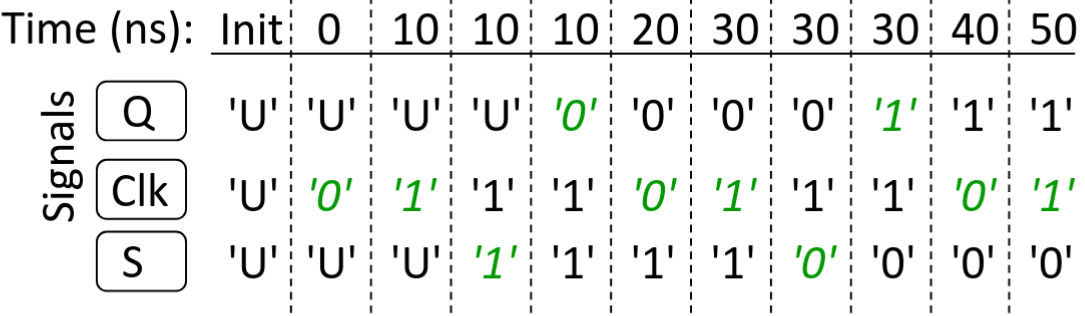
\includegraphics[scale=0.25]{../figures/proc_exec.png}
\end{center}

\textbf{\textsf{Concurrent signal assignments}} can be seen as a sugared version of processes with a single signal assignment.
The sensitivity list is automatically computed from the assignments right hand side arguments.
They are used in dataflow descriptions for:
\begin{itemize}
	\item Descriptions of combinational logic;
	\item Interconnection of components at a lower hierarchical level.
\end{itemize}

For instance, let's look at the example:
\begin{lstlisting}[language=VHDL, style=codestyle]	
ARCHITECTURE Datafl OF fulladder IS
BEGIN
	s  <= (a XOR b) XOR ci;
	co <= (b AND ci) OR (a AND ci) OR (a AND b);
END Datafl;

-- translates to:

ARCHITECTURE Behav OF fulladder IS
BEGIN
PROCESS(a, b, ci)
BEGIN
	s  <= (a XOR b) XOR ci;
	co <= (b AND c) OR (a AND c) OR (a AND b);
END PROCESS;
END Behav;
\end{lstlisting}

\subsubsection{VHDL testbenches}

Once we define an entity, we want to study how our new entity behaves.
We could do this manually, but we have software tools exactly for this reason.
We perform a \textbf{simulation}: User provides input values, simulator generates output values.
\begin{itemize}
	\item A simulation takes in \textbf{test vectors}, that is a sequence of input values;
	\item The result is a \textbf{waveform}, a graphical depiction of the sequence of values the simulation emits.
\end{itemize}

To do this we create new \textbf{testbench} entity that provides test vectors to component's inputs.
An HDL testbench is:
\begin{itemize}
	\item An entity with no ports;
	\item Where we deeclare component to test;
	\item Declare signal for each port;
	\item Instantiate component, map signals to ports;
	\item Process to set signal values at desired times.
\end{itemize}

An example of a testbench can be:
\begin{lstlisting}[language=VHDL, style=codestyle]	
LIBRARY ieee;
USE ieee.std_logic_1164.ALL;

ENTITY Testbench IS
END Testbench;

ARCHITECTURE TBarch OF Testbench IS

    COMPONENT And2 IS
        PORT (
            x : IN  std_logic;
            y : IN  std_logic;
            F : OUT std_logic
        );
    END COMPONENT;

    SIGNAL x_s, y_s, F_s : std_logic;

BEGIN

    CompToTest : And2
        PORT MAP (x_s, y_s, F_s);

    PROCESS
    BEGIN
        -- Test all possible input combinations
        y_s <= '0';
        x_s <= '0';
        WAIT FOR 10 ns;

        y_s <= '0';
        x_s <= '1';
        WAIT FOR 10 ns;

        y_s <= '1';
        x_s <= '0';
        WAIT FOR 10 ns;

        y_s <= '1';
        x_s <= '1';
        WAIT;
    END PROCESS;

END TBarch;
\end{lstlisting}

\subsection{Combinatorial circuits}

A \textbf{circuit}, in the broadest sense, is connection of components.
It's also known as a \textit{structure}.
A circuit is a second way to describe an architecture, in contrast to using a process, as earlier.

When used in a circuit, an entity is known as a \texttt{COMPONENT}.
An \textit{instance} is an occurrence of a component in a circuit.
There may be multiple instances of a component.

This leads us to the third type of concurrent statements: \textbf{component instantiations}.
Let's look at an example:
\begin{lstlisting}[language=VHDL, style=codestyle]	
LIBRARY ieee;
USE ieee.std_logic_1164.ALL;

ENTITY BeltWarn IS -- root entity
    PORT (
        k : IN  std_logic;
        p : IN  std_logic;
        s : IN  std_logic;
        w : OUT std_logic
    );
END BeltWarn;

ARCHITECTURE Circuit OF BeltWarn IS -- root structural description

    COMPONENT And2 IS
        PORT (
            x : IN  std_logic;
            y : IN  std_logic;
            F : OUT std_logic
        );
    END COMPONENT;

    COMPONENT Inv IS
        PORT (
            x : IN  std_logic;
            F : OUT std_logic
        );
    END COMPONENT;

    SIGNAL n1, n2 : std_logic; -- signal declaration

BEGIN -- behavoir starts here

    And2_1 : And2 PORT MAP (k, p, n1);
    Inv_1   : Inv   PORT MAP (s, n2);
    And2_2 : And2 PORT MAP (n1, n2, w);

END Circuit;
\end{lstlisting}

When we create a circuit we have to:
\begin{itemize}
	\item Declare a new entity;
	\item Declare its components.
\end{itemize}

We then want to connect components together.
\textbf{\textsf{Signal}} declaration statements can be useful for this.
A \texttt{SIGNAL} is like a variable in a traditional programming languages: it stores value, but at particular time.
Signals may be explicitly declared, but an entity's ports are also signals.

We use signals in \textit{port maps}.

\textbf{\textsf{Port maps}} are parts of \textit{component instantiations} that map the ports of a component to other ports of the root entity, or signals defined within that entity.

\par\smallskip

At this point some more things about \textit{testbenches} should be clear:
\begin{itemize}
	\item Note use of component instantiation statements;
	\item Signals are used because process cannot access instantiated component's ports directly;
	\item Component instantiation statements and process statements are concurrent statements and they can both appear in an architecture.
\end{itemize}

\textbf{\textsf{Hierarchycal design}}: component instantiation allows for designing entities in an hierarchical manner.
This, alongside generation statements (which we introduced in 2.1.2, and will go in depth afterwards), is going to be one of our most powerful tools for logical design.

To summarize, an entity can be used as component in a new entity.
This process can continue continue: a composed entity can be used as component in another entity, and so on.
This makes hierarchy a powerful mechanism for managing complexity.

\subsection{Top-down design}

Let's introduce the \textbf{top-down} design philosophy.
Designer may initially know system behavior, but not structure.

The idea of top-down design is to:
\begin{itemize}
	\item Capture behavior, and simulate;
	\item Capture structure (circuit), simulate again;
	\item Gets behavior right first, unfettered by complexity of creating structure.
\end{itemize}

How can we describe behavior? One way in VHDL is to use a \textit{process}.
By making a process sensitive to its inputs, the process executes if a change occurs on any of those inputs.
The simplest process uses one signal assignment statement.

We can then simulate the behavior captured by our process using testbench (same as shown earlier) to get waveforms.
We can, this way, proceed to capture structure, simulate again using same testbench.
The result should of course be the same waveforms.

It is useful to have signal assignment statements, as they assign values to signals which can be any combination of different operators.
Note: A port is also a signal.
Lastly, a process may have multiple signal assignment statements.

We will now cover a few more constructs which can be useful to capture high level behavior.

\textbf{\textsf{If statements}} are supported by VHDL. The condition \textit{has} to be boolean, and errors will be reported at compile time.

We see an example:
\begin{lstlisting}[language=VHDL, style=codestyle]	
LIBRARY ieee;
USE ieee.std_logic_1164.ALL;
ENTITY BeltWarn IS
	PORT (
		k, p, s : IN std_logic;
		w : OUT std_logic
	);
END BeltWarn;
ARCHITECTURE Behav OF BeltWarn IS
BEGIN
	PROCESS (k, p, s)
	BEGIN
		IF ((k AND p AND NOT(s)) = '1') THEN
			w <= '1';
		ELSE
			w <= '0';
		END IF;
	END PROCESS;
END Behav;
\end{lstlisting}

\texttt{ELSIF} is also supported, in Python fashion.

\textbf{\textsf{Vectors}} are provided by \texttt{std\_logic\_vector}.
These represent collection of bits, which is more convenient than declaring separate bits like \texttt{d3, d2, d1, d0}.
A nice feature is that a vector's bits are numbered: the ordering is specified in the syntax: \texttt{(0 TO 3)}, \texttt{(1 TO 4)}, ...
Assignment is possible with strings of bits.

An example is:
\begin{lstlisting}[language=VHDL, style=codestyle]	
LIBRARY ieee;
USE ieee.std_logic_1164.ALL;

ENTITY Dcd2x4vect IS
	PORT (i: IN std_logic_vector(0 TO 1);
		  d: OUT std_logic_vector(0 TO 3);
END Dcd2x4vect
\end{lstlisting}

\textbf{\textsf{Switch statements}} are also available, and they are called \texttt{CASE} statements.
These are preferred over \texttt{IF-THEN-ELSE} when a single expression determines which
statement(s) to execute.
The selection keyword is \texttt{WHEN}, and the sequence of statements after a \texttt{WHEN} includes all statements between the \texttt{WHEN} itself and the next \texttt{WHEN} or \texttt{END CASE}.

An example is:
\begin{lstlisting}[language=VHDL, style=codestyle]	
ARCHITECTURE Dcd2x4_vect OF Dcd2x4vect IS
BEGIN
	PROCESS (i)
	BEGIN
		CASE i IS
			WHEN "00" => d <= "0001";
			WHEN "01" => d <= "0010";
			WHEN "10" => d <= "0100";
			WHEN OTHERS => d <= "1000";
		END CASE;
	END PROCESS;
END Dcd2x4_vect
\end{lstlisting}

The \textit{case sequential} statement is allowed, that is a \texttt{WHEN} clause can include more than one choice:
\begin{lstlisting}[language=VHDL, style=codestyle]	
CASE expression IS
	WHEN choices =>
		-- sequential statements
	WHEN choices =>
		-- sequential statements
		-- (branches are allowed)
	WHEN OTHERS =>
		-- sequential statements	
END CASE;
\end{lstlisting}

\subsection{Design units}

VHDL allows for \textbf{design units}.
They are VHDL code segments that can be compiled separately and stored in a library for future use.
Libraries are collections of compiled design units that are mapped to physical directories.A library is a set of components (entities and architectures) and packages.

There are 5 types of design units:
\begin{enumerate}
	\item Entity;
	\item Architecture;
	\item Package;
	\item Package body;
	\item Configuration.
\end{enumerate}

\subsubsection{Packages}

\textbf{Packages} are repositories for type definitions, procedures and functions.
They group common declarations used by several design units.
Standard packages are defined in generic libraries (e.g. IEEE) for numeric/text handling (for example, \texttt{std\_logic\_1164}, \texttt{numeric\_std}, \texttt{std\_logic\_arith}, \texttt{std\_logic\_signed}, \texttt{std\_logic\_unsigned}, TEXTIO, ...).

A package consists of:
\begin{itemize}
	\item A package \textbf{declaration} (with declarations of types, subtypes, constants, global signals, functions and procedures, attributes, files, components, ...).

	      Because a package serves as a central repository for frequently used utilities, such as component declarations, ... the declarations may then be reused by any VHDL model by simply accessing the package.

	      Usually, to use a package we use the \texttt{USE} clause.

	      An example of a package declaration is:
	      \begin{lstlisting}[language=VHDL, style=codestyle]	
PACKAGE example IS
	TYPE winter IS (Dec, Jan, Feb);
	COMPONENT And3 IS
		PORT (
			x : IN std_logic;
			y : IN std_logic;
			z : IN std_logic;
			F : OUT std_logic
		);
	END COMPONENT;
	CONSTANT pin2pin_delay : TIME := 125ns;
	FUNCTION int2bit_vect (int_val : INTEGER) RETURN bit_vector;
END example;
\end{lstlisting}
	\item A package \textbf{body}: it contains the implementations of functions, procedures, ... A package body is always associated with a package declaration.

	      An example of a package body is:
	      \begin{lstlisting}[language=VHDL, style=codestyle]	
PACKAGE BODY example IS
	FUNCTION int2bit_vect (int_val : INTEGER) RETURN bit_vector IS
		BEGIN
			-- behavior of function described here
		END int2bit_vect;
END example;
\end{lstlisting}
\end{itemize}

\subsubsection{Configurations}

VHDL description may consist of many design entities, each with several architectures, and organized into a design hierarchy.
A \textbf{configuration} does the job of specifying the exact set of entities and architectures used in a particular simulation or synthesis run.

A configuration does two things:
\begin{itemize}
	\item It specifies the design entity used in place of each
	      component instance (i.e., it plugs the chip into the chip
	      socket and then the socket-chip assembly into the
	      PCB);
	\item It specifies the architecture to be used for each design
	      entity (i.e., which die).
\end{itemize}

A configuration statement is used to bind a component instance
to an entity-architecture pair. A configuration can be considered
as a parts list for a design. It describes which behavior to use for
each entity, much like a parts list describes which part to use for
each part in the design.

Component configuration can be performed outside the
architecture body which instantiates a certain component.
A configuration declaration is a design unit which can be
compiled separately.
The particular architecture body has not to be recompiled when
the binding is changed.

\subsubsection{Libraries}

\textbf{Libraries} are collections of compiled design units that are mapped to
physical directories. A library is a set of components (entities and
architectures) and packages.

There are two reserved library names always available to designers:
\begin{itemize}
	\item \texttt{work}: predefined library;
	\item \texttt{STD}: it contains 2 packages:
\begin{itemize}
	\item \texttt{STANDARD} provides declaration for predefined types (real, integers, Boolean, etc);
	\item \texttt{TEXTIO} contains useful subprograms that enables to perform ASCII file manipulation.
\end{itemize}
\end{itemize}

The statement \lstinline|library STD;| declares STD to be a library.
The statement \lstinline|USE STD.STANDARD.ALL;| allows the use of all declarations in package \texttt{STANDARD} located within the library \texttt{STD}.
The statement \lstinline|LIBRARY ieee;| declares \texttt{ieee} to be a library. \texttt{work} is the predefined library.

\end{document}
